\documentclass{article}
\usepackage[utf8]{inputenc}
\usepackage{geometry}
\usepackage{fullpage}
\usepackage{ctex}
\usepackage{float}
\usepackage{graphicx}
\usepackage{subfigure,float}

\usepackage{algorithm}
\usepackage{algorithmicx}
\usepackage{algpseudocode}

\usepackage{hyperref, wrapfig,fancybox,listings,subfigure}

\lstset{numbers=left,
keywordstyle=\color{blue!70}, commentstyle=\color{red!50!green!50!blue!50},
frame=shadowbox,
rulesepcolor=\color{red!20!green!20!blue!20},
breaklines=true,
extendedchars=true
}

\title{高等计算机图形学大作业:三维造型与渲染}
\author{王世因 2016011246}
\date{}
\begin{document}
\maketitle

\tableofcontents
\newpage


\section{得分点}

\begin{itemize}
\item 三角网格求交(Object.hpp \& Object.cpp)
\item 参数曲面求交(Object.hpp \& Object.cpp)
\item 随机渐进光子映射(SPPM.hpp \& SPPM.cpp)
\item KD Tree加速(KDTree.hpp \& KDTree.cpp)
\item AABB包围盒加速(AABB.hpp \& AABB.cpp)
\item OpenMP加速(SPPM.hpp \& SPPM.cpp)
\item 景深(SPPM.cpp)
\item 贴图(Texture.hpp \& Texture.cpp)
\item 超采样
\end{itemize}

\section{算法原理}

在本学期的课堂上,我们介绍了许多真实感图像生成的算法,通过建模真实世界中的光学过程来渲染出逼真的图片效果。在我看来,建模可以从两个角度切入,一个是从物体开始搜索相机,一个是从相机开始搜索看到的物体。我选择了原理上更吸引我的渐进光子映射算法,采用了随机化的实现方式(SPPM随机渐进光子映射)。在物体的建模上我采用了三角网格求交和Bezier参数曲面求交的两种方式,均衡了效果和计算速度。

\subsection{随机渐进光子映射(SPPM)}

我在本次大作业中选择的是随机渐进光子映射的算法,在每一轮迭代中,从相机通过成像平面的各个点确定一条光线,然后运行光线追踪的算法,光线根据概率被吸收、反射和折射,在光线被吸收或者超过迭代次数后返回空间中对应的点。意思是,找到我们在视野中看到的究竟是哪一个点,在渐进光子映射中,我们只运行一遍刚才所描述的构建Hitpoint数组的代码,而在随机渐进光子映射中,每一轮都要进行这个操作,一方面是添加了随机的扰动,另一方面也给概率化地构建光线追踪随机吸收、反射和折射的模型提供了可能。具体的代码分布在Scene和SPPM中,已经进行了相关的注释。


\subsection{参数曲面求交}
在老师上课的时候将了很多工业界的曲面建模手段,比如Bezier和B样条这种比较通用的。这里我想做一个比较好看的水滴状的物体,难点在于底部需要十分平滑才美观,虽然说Bezier参数曲面可以控制住旋转体的导数,但是直接解参数曲面是我看来比较好的方法。我选择了著名的Teardrop Curve来旋转:

\begin{figure}[H]
\centering
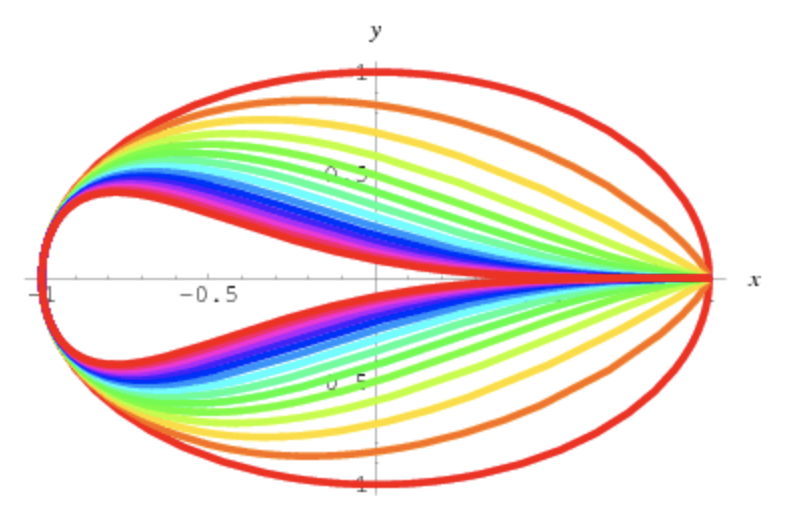
\includegraphics[scale=1]{3.png}
\end{figure}

\begin{equation}
x = cos(t)
\end{equation}

\begin{equation}
y = sin(t)sin^m(\frac{t}{2})
\end{equation}

这里我取$m=2$的曲线,将水滴的简短指向y轴正方向,并扩展到三维的旋转体后就可以得到下面的简化版本:

\begin{equation}
x^2+z^2 = y(y-1)^2
\end{equation}

如果设光线从它的源头传播到和参数曲面碰撞经过的路程是$t$,因为光线的源头和方向已知,我们可以得到一个仅和$t$有关的参数方程。求出方程的系数后就可以直接用不动点迭代法解决了。利用包围盒我们可以提升一下这部分的计算效率。

\begin{equation}
2\sqrt{x^2 + z^2} = \frac{\partial y}{\partial \sqrt{x^2 + z^2}}(3y-1)(y-1)
\end{equation}

因此我们可以求得曲面的法向量。


%\subsection{KD Tree}


%\subsection{贴图}



%\subsection{网格简化}


%\subsection{图片降噪}



\section{实验结果}

\subsection{透镜成像}

\begin{figure}[H]
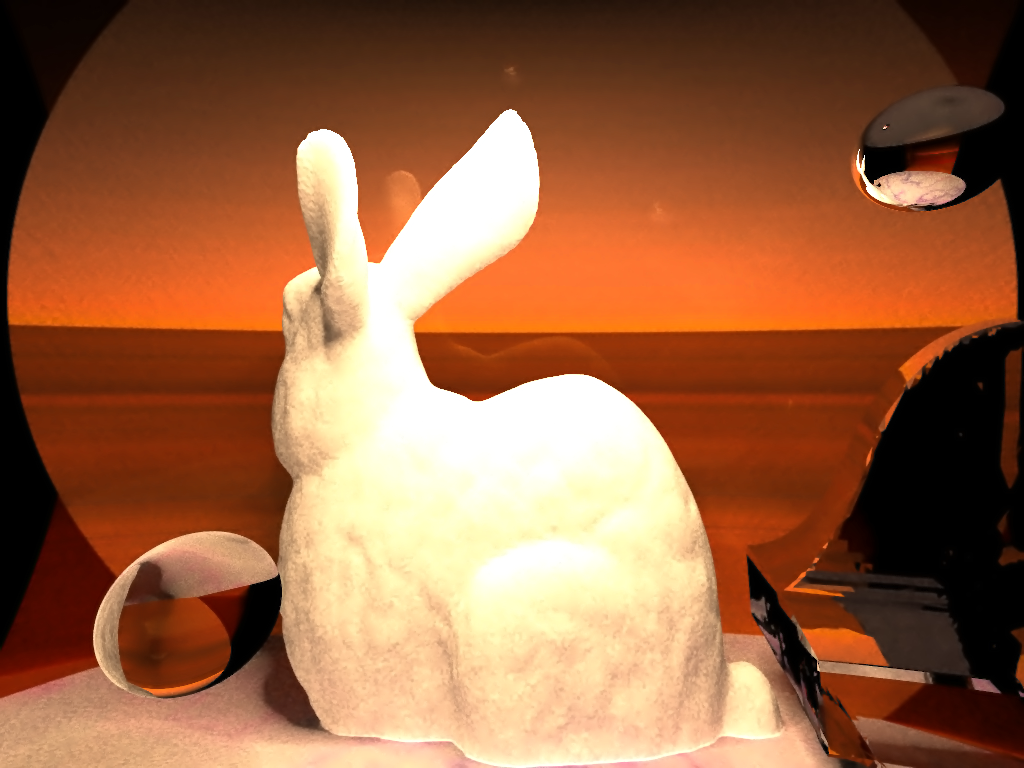
\includegraphics[width=\columnwidth]{1.png}
\end{figure}

这是我认为最有意思的一张图,相机和物体之间有一个巨大的圆球,这个圆球充当了透镜的作用,针对圆球背面的圆形平面贴图营造出一种窗户的效果,有一种玉兔在看窗外月球落日的意境。这里的两个球因为透镜的效果变形了,比参数曲面生成的类似几何造型更容易渲染。

\subsection{Box全景视图渲染}

\begin{figure}[H]
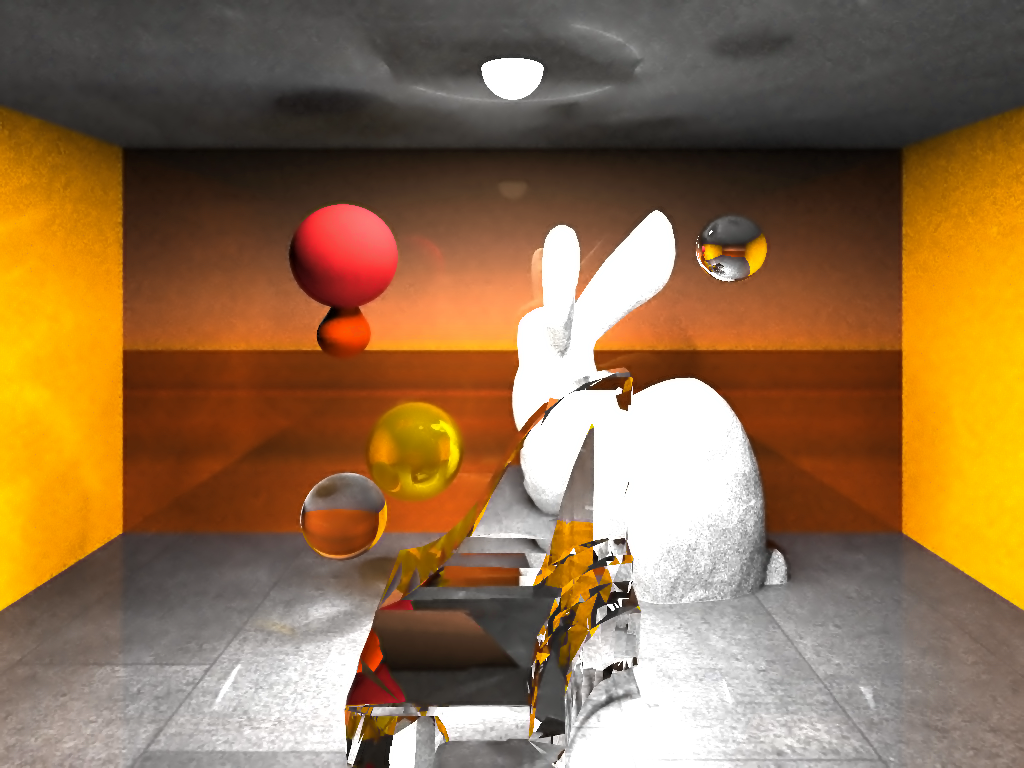
\includegraphics[width=\columnwidth]{2.png}
\end{figure}

因为要体现出{\bf{随机渐进光子映射}}的效果,我在选择了一个棱角结构复杂的玻璃材质的废墟素材放到光源下,头顶的球形光源折射进入玻璃在地板上有许多的光斑产生,也在天花板上反射了许多的光斑。

这张图也能体现出{\bf{景深}}的效果,镜头聚焦在前景的玻璃废墟上,后面的黄色大球边缘变得模糊。

另外,四个小球体现了反射、折射和阴影的效果。我借鉴了很多网上的资料,让光线依概率反射、折射、吸收,利用参数模拟出各种材质。

红色的大球下的那个小水滴状的东西就是我用{\bf{参数曲面}}生成的Teardrop Curve。











\end{document}